\begin{multicols}{3}[\section{Bluetooth Low Energy}]

\rhead{Sven Guthe, Lucas Lorenz}
\lfoot{16.05.2016}

\newrefsegment

\begin{tabular}{p{2,1 cm}p{2.7 cm}}
\textbf{Steckbrief}& \\
\end{tabular}
\rowcolors{1}{\topicolor!20}{}
\begin{tabular}{p{2,1 cm}p{2.7 cm}}
      Einsatz seit & Dezember 2009\\
      Frequenz"-bereich  & \SI{2,4}{\giga\hertz}-Band mit 40 Kanälen zwischen \SI{2,402}{\giga\hertz} und \SI{2,483}{\giga\hertz}\\
      Datenrate & \SI{0,27}{Mbit/s}\\
      Verbreitung & Weltweit (vor allem Smart Wearables)\\
      Reichweite & \SI{10}{\metre}\\
\end{tabular}

\par
\subsection*{Überblick}
\begin{wrapfigure}{r}{0.4\linewidth}
  \vspace{-20pt}
  \begin{center}
  	\hspace{-20pt}
    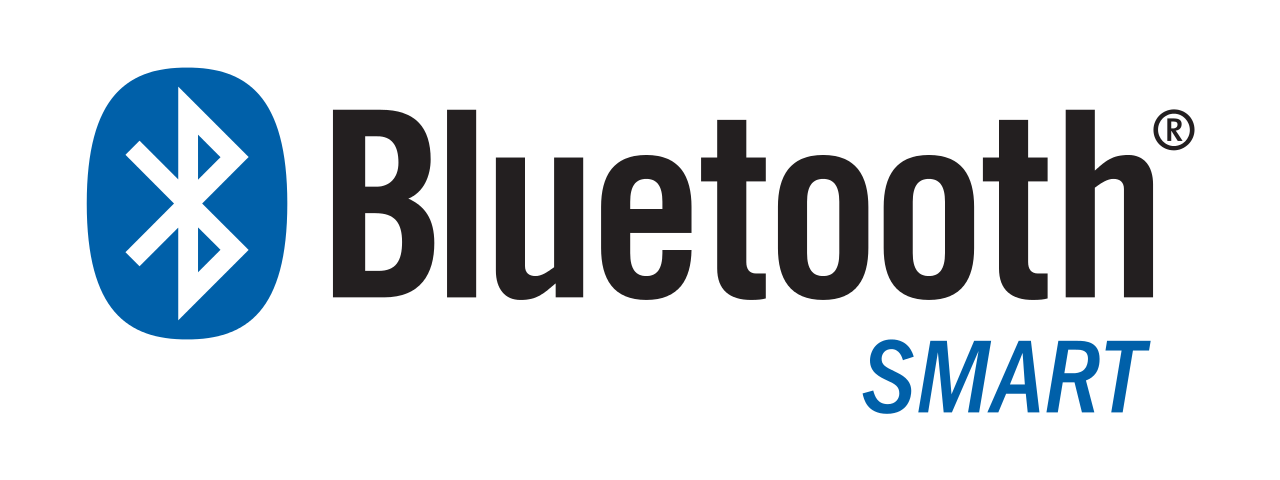
\includegraphics[width=0.7\linewidth]{Kapitel/BLE/Grafiken/Bluetooth_Smart_Logo.png}
    %\captionof{figure}{Bluetooth Smart Logo~\cite{BLE.2}}
  \end{center}
  \vspace{-15pt}
\end{wrapfigure}
\textit{\textbf{B}luetooth \textbf{L}ow \textbf{E}nergy} (\textbf{BLE}) ist eine kabellose Übertragungstechnologie, welche für Datenübertragungen auf kurzen Entfernungen von der \textit{Bluetooth \textbf{SIG}} (\textbf{S}pecial \textbf{I}nterest \textbf{G}roup) entwickelt wurde. Es handelt sich hierbei um eine Bluetooth-Spezifikation, bei welcher der energiesparende Betrieb im Vordergrund steht, um Verbindungen zu Geräten mit kleinem Energiespeicher herzustellen. Mit dieser Entwicklung, sichert sich der Bluetooth-Standard vor allem in den aufstrebenden Märkten der Gesundheitsindustrie und der Unterhaltungselektronik Anteile. In diesen Bereichen kann die Technologie beispielsweise in Fitnesstrackern und Kopfhörern eingesetzt werden. 
%Gesundheitsindustrie, hier zum Beispiel in Fitnesstrackern, und in Geräten der Unterhaltungselektronik wie Kopfhörern.
Zur Anwendung kommt BLE in Wearables wie Smartwatches, in Notebooks, Smartphones und in vielen weiteren Geräten~\cite{BLE.4}.
\subsection*{Technische Erläuterungen}
\begin{Figure}
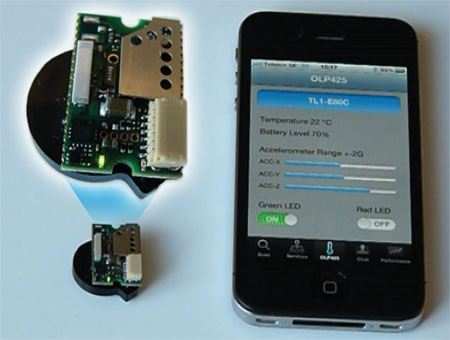
\includegraphics[width=\linewidth]{Kapitel/BLE/Grafiken/BLE_mod.jpg}
\captionof{figure}{Bluetooth-Module im iPhone 4S~\cite{BLE.6}}
\label{fig:BLE-Mod}
\end{Figure}
Eine Bluetooth-Verbindung basiert auf der Kommunikation zwischen einem \textit{Master} und einem \textit{Slave}. Der Master ist dabei das Gerät, welches die Verbindung initiiert. Dieser stellt auf 40 Kanälen eine Verbindung zum Slave her und kann dank des Frequenzsprungverfahren auf allen Kanälen parallel Daten senden, wodurch die Bandbreite enorm erhöht wird. Als Konsequenz ergibt sich, dass alle verbundenen Slave-Geräte mit dem Takt des Masters synchronisiert werden müssen.
Eine Verbindung des Masters zu mehreren (max. 7) Slaves wird als \textit{Piconet} bezeichnet. Befindet sich ein Gerät in mehreren Piconets, wird dies \textit{Skatternet} genannt. Bei diesen Netzen kommt es zusätzlich zur Abstimmung der jeweiligen Sendekanäle und der Reihenfolge, in welcher die Daten in das jeweilige Piconet gesendet werden.

Wie es auch bei der Datenübertragung von vielen anderen Techniken geschieht, werden die zu übersendenden Daten in Pakete unterteilt und in diesen Einheiten versendet. Dabei wird bei dem Bluetooth Standard unterschieden zwischen einer synchronen (\textbf{SCO} - \textbf{s}ynchronous \textbf{c}onnection \textbf{o}riented) und in einer asynchronen (\textbf{ACL} - \textbf{a}synchronous \textbf{c}onnection\textbf{l}ess) Übertragung. Für die BLE-Technologie ist dabei vor allem die asynchrone Übertragung von Interesse. Dabei werden Daten zu einem beliebigen Zeitpunkt über die Piconets versendet und können gegebenenfalls erneut angefordert werden.
\begin{Figure}
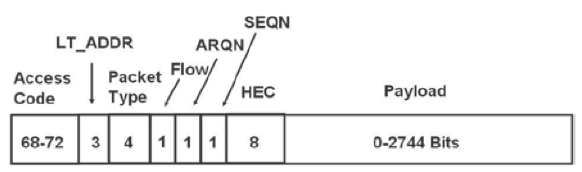
\includegraphics[width=\linewidth]{Kapitel/BLE/Grafiken/paket.png}
\captionof{figure}{ACL Paket~\cite{BLE.1}}
\label{fig:BLE-ACL-Paket}
\end{Figure}
%Flags wirkt wirr
Ein ACL-Datenpaket bestehet aus einer Identifikationssequenz (68-72 Bit, Access Code) zur Identifikation für das aktuelle Piconet, aus der Adresse des Slaves (3 Bit, Logical Transfer Address), einer Information über den verwendeten Pakettyp (4 Bit, Packet Type), 3 Flags, welche für das Blockieren des Controllers (Flow), für die Information, ob das letzte Paket erfolgreich angekommen ist (Automatic Repeat Request Number) und einer \textbf{Seq}uenz\textbf{n}ummer (\textbf{SEQN}), um zu überprüfen, ob die Reihenfolge eingehalten wurde, stehen. Außerdem wird ein Hashwert (8 Bit, Header Error Check) angefügt, um ein mögliches falsches Paket zu erkennen. Hinter dieser festgesetzten Folge von Bits folgen schließlich die eigentlichen Informationen mit  0-2744 Bits, wobei nochmals 32 Bits für konkrete Informationen zum Paket verloren gehen (vergl. Abb. \ref{fig:BLE-ACL-Paket}).
%Das steht schonmal irgendwo weiter oben? 
\begin{Figure}
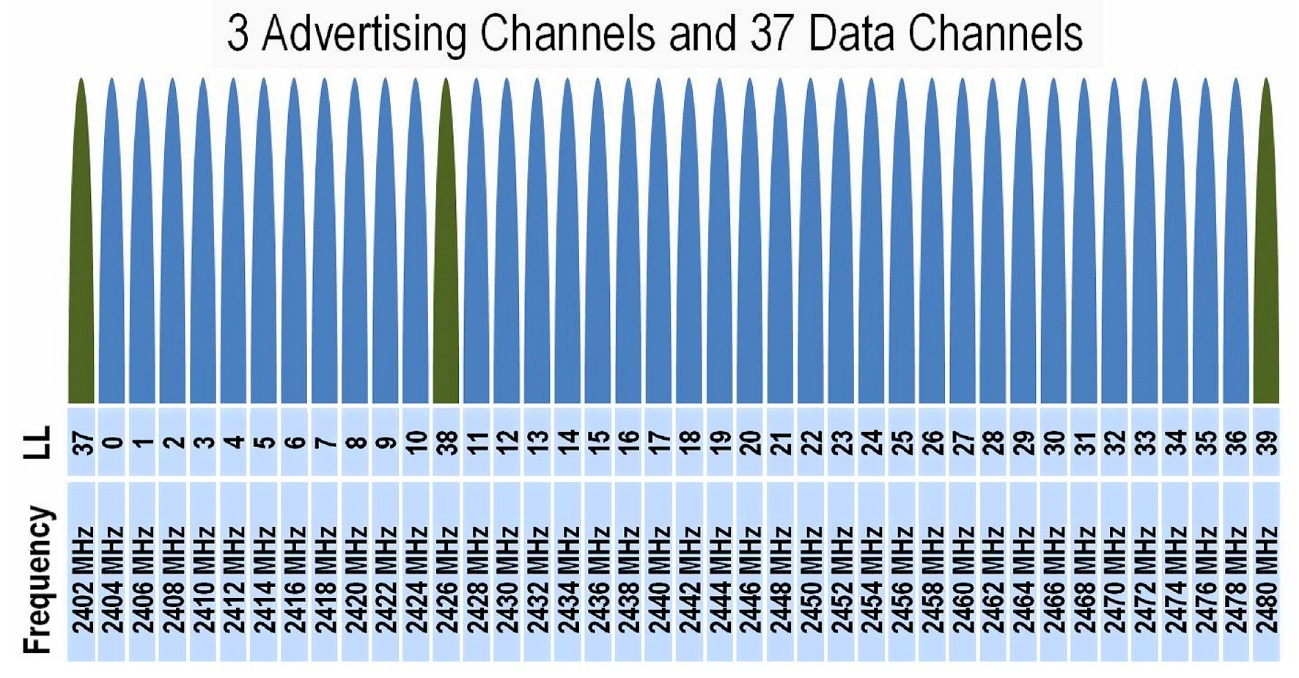
\includegraphics[width=\linewidth]{Kapitel/BLE/Grafiken/BLE_DC.jpg}
\captionof{figure}{Kanäle im BLE-Frequenzbereich~\cite{BLE.7}}
\label{fig:BLE-DC}
\end{Figure}
Die Datenübertragung findet dabei auf 40 Kanälen im Frequenzbereich zwischen \SI{2,402}{\giga\hertz} und \SI{2,483}{\giga\hertz} statt (siehe Abb. \ref{fig:BLE-DC}). Damit kommt es zwar zwischen BLE und anderen Funktechnologie zu Überlagerungen, allerdings wechselt BLE seinen Sendekanal bis zu 1600 mal pro Sekunde.
Um die Übertragung entsprechend zu modulieren, wird der \textbf{GFSK}-Standard (\textbf{G}aussian \textbf{F}requency \textbf{S}hift \textbf{K}eying) eingesetzt, bei der die schnell und stark ansteigenden Flanken abgeflacht und somit die für die Übertragung weniger Bandbreite benötigt wird.

Für die Übertragung werden Protokolle verwendet, welche jenen aus dem bekannten OSI-Modell entsprechen. Dabei kommen die Schichten des Physical Layers in Form des \textit{Radio Layers} und der Data Link Layer in Form des \textit{Baseband} und des \textit{Link Manager Layers} zum Einsatz. 
Der Radio Layer übernimmt die Modulation sowie die Demodulation des Signals und versendet bzw. empfängt physikalische Signale. Der Baseband Layer sorgt für die Kontrolle der angekommenen Daten und sendet, falls nötig, eine Aufforderungen zur erneuten Sendung von fehlgeschlagenen Paketen. Zuletzt analysiert und verwaltet der Link Manager Layer alle Verbindungen und setzt eine Authentifizierung zwischen Master und Slave sowie eine Verschlüsselung um.

%letzter satz klingt holprig
Bezüglich der Authentifizierung lässt BLE die Möglichkeiten offen, ob diese stattfinden muss oder nicht. Mithilfe des \textbf{OPP} (\textbf{O}bject \textbf{P}ush \textbf{P}rofile) können Daten auch ohne Authentifizierung gesendet werden. Am Slave-Gerät muss hierbei nur bestätigt werden, dass die Daten angenommen werden. Allerdings entspricht dies nicht dem Normalfall.
Wie bei dem Serial Port Profile müssen sich Geräte vor einer Datenübertragung pairen. Dazu ist es notwendig einen zuvor ausgehandelten Schlüssel, eine PIN, einzugeben. Nach erfolgreichem Pairing, wird das verbundene Gerät in eine Liste von bekannten Geräten aufgenommen. Neben dem Einsatz von PINs, wird auch das Pairing per \textbf{NFC} (\textbf{N}ear \textbf{F}ield \textbf{C}ommunication) immer verbreiteter.

%stromsparender Verbrauch? größter Unfug ever
Das Spezielle am Bluetooth Low Energy Standard sind die genutzten Zeitintervalle und die Datenmenge, welche an gekoppelte Geräte übertragen werden. Anders als bei allen anderen Bluetooth-Standards ist, dass BLE auf den Geräten nicht dauerhaft eingeschaltet ist, sondern nur in gewissen Zeitabständen relevante Informationen sendet. Außerdem ist auch die Datenübertragung in ihrem Umfang eingeschränkt. Es werden maximal 220 kBit/s übertragen. Dies bedeutet, dass BLE nicht für alle Anwendungen in Frage kommt und bei größeren Datenmengen doch auf andere Standards zurückgegriffen werden muss. Durch den Fokus auf den stromsparenden Verbrauch von Bluetooth, wird neben der Datenrate und den Zeitabständen auch die Reichweite stark eingeschränkt. Von rund 100 Metern bei "normalen" Bluetooth sind bei BLE lediglich 10 Meter zu erreichen~\cite{BLE.1}.
\subsection*{Einsatz}
\begin{Figure}
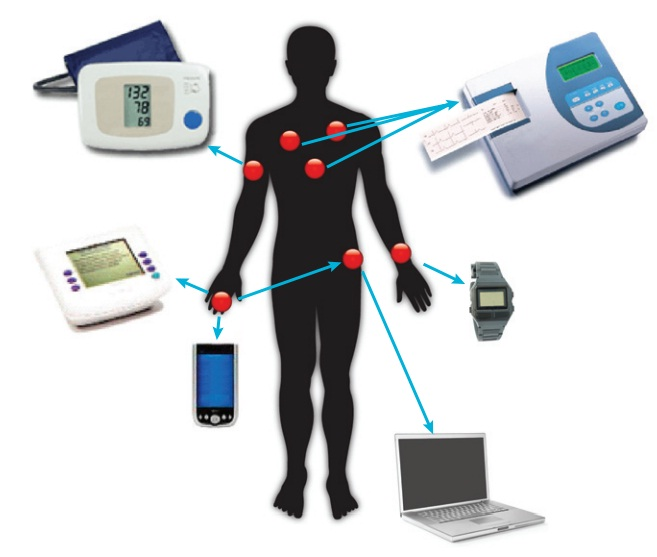
\includegraphics[width=\linewidth]{Kapitel/BLE/Grafiken/BLE_Use}
\captionof{figure}{Einsatzmöglichkeiten von BLE~\cite{BLE.5}}
\label{fig:BLE.use}
\end{Figure}
Die Einsatzmöglichkeiten von BLE sind sehr breitgefächert. Dabei wird auf einzelne Anwendungsgebiete genauer eingegangen, wie sie auch zum Teil aus Abb. \ref{fig:BLE.use} hervorgehen. 

%wirklich? durchaus?
Ein durchaus gewinnbringender Einsatz ist im Einzelhandel möglich. Dabei können Geräte des Kunden im Geschäft automatisch Kontakt zu einem Bluetooth Access Point aufnehmen und Informationen über den Kunden und dessen Kaufverhalten an die Verkäufer senden. 
\end{multicols}
\section*{Historische Entwicklung}
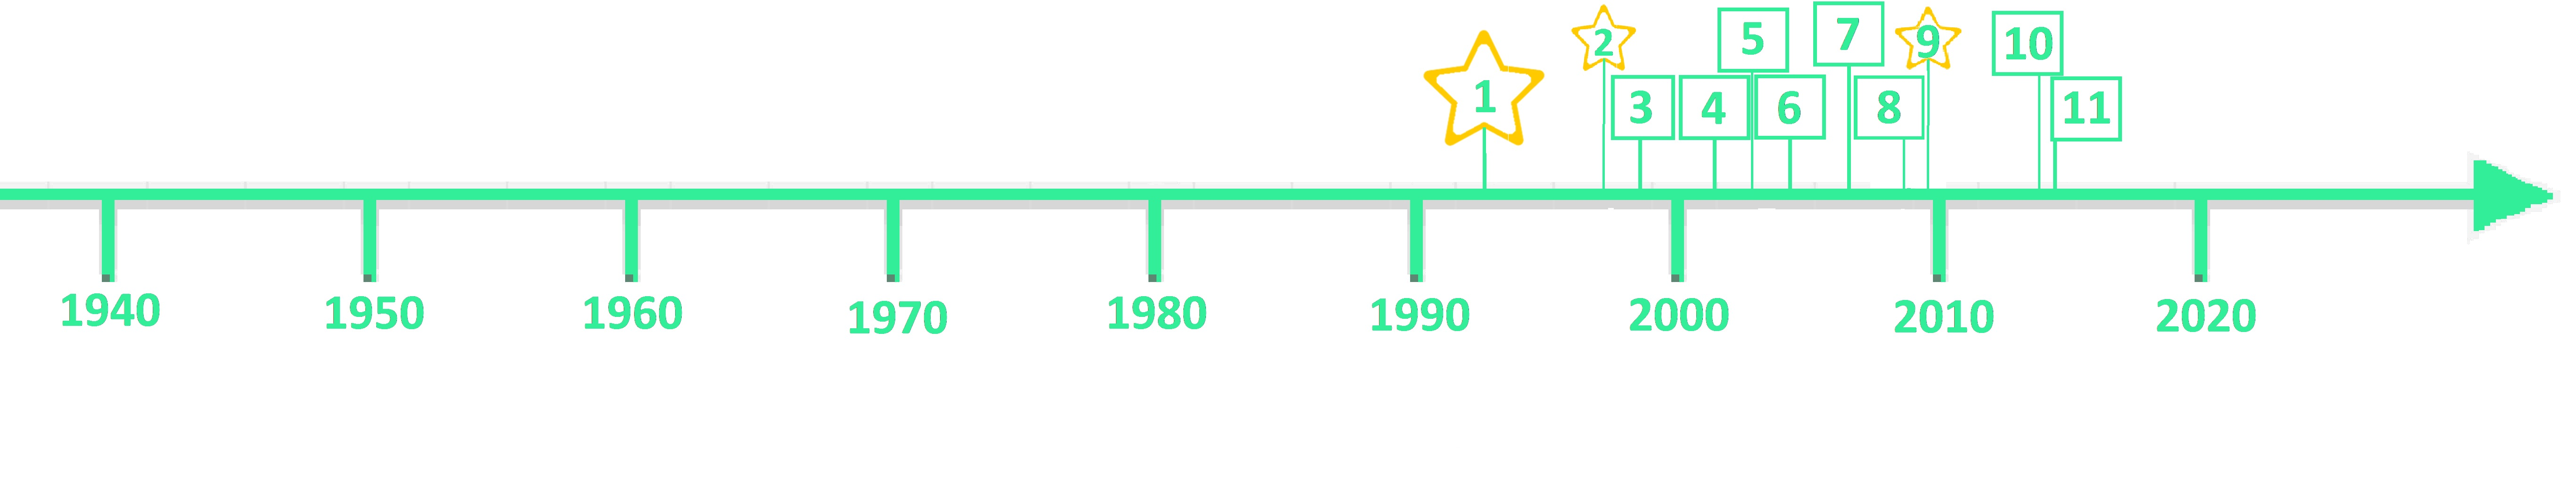
\includegraphics[width=\textwidth]{Kapitel/BLE/Grafiken/Zeitstrahl}
\par
\noindent
\rowcolors{2}{}{\topicolor!20}
\begin{tabular}{p{0.5 cm}p{3 cm}p{13.55 cm}}
	Nr. & Datum & Information \\
	1 & August 1993 & Gründung der \textbf{IrDA} (\textbf{I}nfra\textbf{r}ed \textbf{D}ata \textbf{A}ssociation) mit dem Ziel ein einheitliches Protokoll für Datenübertragung über Infrarot bereitzustellen.\\
	2 & 1998 & Gründung der Bluetooth SIG durch die Firmen \textit{Ericsson, Nokia, IBM, Toshiba} und \textit{Intel} zur Ausarbeitung eines Standards, der verbindliche Spezifikationen festlegte.\\
	3 & Juli 1999 & Bereitstellung der Spezifikation Bluetooth 1.0 (Juli) und Bluetooth 1.0b (Dezember).\\
	4 & Februar 2001 & Bereitstellung der Spezifikation Bluetooth 1.1.\\
	5 & November 2003 & Bereitstellung der Spezifikation Bluetooth 1.2.\\
	6 & November 2004 & Bereitstellung der Spezifikation Bluetooth 2.0 + EDR.\\
	7 & August 2007 & Bereitstellung der Spezifikation Bluetooth 2.1 + EDR.\\
	8 & April 2009 & Bereitstellung der Spezifikation Bluetooth 3.0 + HS.\\
	\textbf{9} & \textbf{Dezember 2009} & \textbf{Bereitstellung der Spezifikation Bluetooth 4.0.}\\
	10 & Dezember 2013 & Bereitstellung der Spezifikation Bluetooth 4.1.\\
	11 & Dezember 2014 & Bereitstellung der Spezifikation Bluetooth 4.2.\\
\end{tabular}
\par
\begin{multicols}{3}
Interessante Informationen wären dabei Browserverläufe, bei denen sich der Kunde auf der Suche nach Mode befand, vorausgesetzt der Kunde befindet sich in einem Modegeschäft. Neben den Möglichkeiten, den Verkäufer mit relevanten Informationen zu versorgen, ist es natürlich ebenfalls möglich, dem vermeintlichen Käufer einen Überblick über den Laden zu geben und benötigte Kleidung zu lokalisieren.

Das aber vermutlich gewinnbringendste Gebiet für BLE ist die Gesundheitsbranche. Geräte zum Puls anzeigen, Schritte zu zählen oder auch Sportaktivitäten aufzuzeichnen sind bereits überall in allen Preisklassen erhältlich. Aber die Branche wird noch viel weiter gehen. Warum sollten nicht auch detailliertere Informationen über den Zustand des Körpers ermittelt und an das Handy oder gar direkt ans zuständige Krankenhaus gesendet werden? Mit kleinen Sensoren, welche über ein Modul für BLE verfügen, wäre dies realisierbar und stellt auch für den Nutzer einen Mehrwert dar, da er sich jeder Zeit über den Zustand seines Körpers informieren kann und ihm anhand dieser Daten gegebenenfalls eine genauere oder schnellere Diagnose im Krankheitsfall gestellt werden kann.

%exisitiert doch schon?
Auch in der Industrie bei der Wartung von Maschinen ist ein Verwenden von Bluetooth von großem Vorteil. Damit wäre es möglich, Fehler unabhängig von der Maschine mit einem einzelnen portablen Gerät (Handy) abzulesen. Dadurch würden die Unternehmen unabhängiger von teurer Software der Entwickler und könnten die Oberflächen je nach Anwendungsbedarf selbst modifizieren.
%klingt unlogisch

Wie schon durch die drei aufgelisteten Beispiele zu erkennen ist, ist Bluetooth in allen Gebieten des Lebens verwendbar in denen Daten übertragen werden müssen. Durch das Entwickeln des BLE Standards ist man zudem unabhängiger von Entwicklungen in der Batterieindustrie und kann mittels kleiner Energievorräte, Daten an kompatible Geräte senden.

Damit wird BLE nicht nur für Konsumenten einen Mehrwert darstellen, sondern auch in der Entwicklung des \textit{Internet der Dinge} (\textbf{IoT} - \textbf{I}nternet \textbf{o}f \textbf{T}hings) in Verbindung mit SmartHome und anderen Technologien~\cite{BLE.1}.
%entspricht tabelle --> vermutlich firmen aus tabelle herausnehemn
\subsection*{Anbieter und Gremien}
Das Gremium, welches für die Entwicklung von neuen Bluetooth-Technologien zuständig ist, ist die schon genannte Bluetooth SIG. Gegründet wurde dieses Gremium 1998 von den Unternehmen \textit{Nokia, Toshiba, Intel, IBM} und \textit{Ericsson}. Bis zum Jahre 1999 stiegen auch \textit{3Com, Motorola, Lucent} und \textit{Microsoft} in die SIG ein. Die Interessengruppe besitzt das Warenzeichen von Bluetooth und bestimmt mit den Entwicklungen der neuen Standards auch deren Spezifikationen. Mittlerweile wird die SIG Gremium von mehr als 30.000 Mitgliedern unterstützt~\cite{BLE.1}.
%bild austauschen, weil 0.000 Informationsgehalt
\begin{Figure}

\includegraphics[width=\linewidth]{Kapitel/BLE/Grafiken/BluetoothSIGLogo.jpg}
\captionof{figure}{Bluetooth SIG Logo~\cite{BLE.3}}
\end{Figure}
\subsection*{Ausblick}
%umformulieren und ggf ausbauen, IT 4.0 -- je nach bildern vorne
Einen kleinen Ausblick konnte man schon aus den möglichen Einsatzgebieten ableiten, woraus auch hervorgeht, wie wichtig Bluetooth in der zukünftigen Vernetzung sein wird. Neben den Anwendungsgebieten, welche mit besseren Eigenschaften natürlich auch weiter steigen, sind auch neue Standards mit höheren Übertragungsraten im Low Energy Bereich geplant. Damit wird der BLE Standard auch für Anwendungen, in denen mehr Datenvolumen übertragen werden muss, interessant.

Das größte, interessanteste, aber auch unberechenbarste Gebiet der Entwicklung für Übertragungstechnologie wird allerdings das Internet der Dinge darstellen. In der immer schnelleren Vernetzung des eigenen Zuhauses, des Körpers und andere Dinge des täglichen Lebens werden Übertragungsmöglichkeiten zwischen den Sensoren immer wichtiger. Ob sich der Bluetooth Standard dabei durchsetzt ist aufgrund der Schnelllebigkeit in Gebieten der Technik allerdings nicht zu beurteilen~\cite{BLE.1}.

\printbibliography[segment=13,heading=subbibliography]
\end{multicols}

\newpage
